\documentclass[a4paper,12pt,openany]{article}
\usepackage[utf8]{inputenc}
\usepackage[vietnamese]{babel}
\usepackage{fancyhdr}
\usepackage{float}
\usepackage{geometry}
\usepackage{caption}
\usepackage{amsmath} 
\usepackage{amssymb} 
\usepackage{amsfonts} 
\usepackage{tabularx}
\usepackage{graphicx}
\usepackage{listings}

\title{Report - week 3}
\author{Le Xuan Duan}


%Căn lề cho văn bản 
\geometry{ 
        left=3cm, % Lề trái 
        right=3cm, % Lề phải 
        top=2.5cm, % Lề trên 
        bottom=2.5cm, % Lề dưới 
        headheight=15pt, % Chiều cao phần đầu trang 
        headsep=1cm, % Khoảng cách từ phần đầu trang đến phần nội dung 
        }
        
\setlength{\parindent}{0pt}
\captionsetup{margin=40pt}
\captionsetup{labelfont=bf}

\begin{document}

\maketitle
\section{Warm up - Exercise week 3}
\begin{figure}[H]
    \centering
    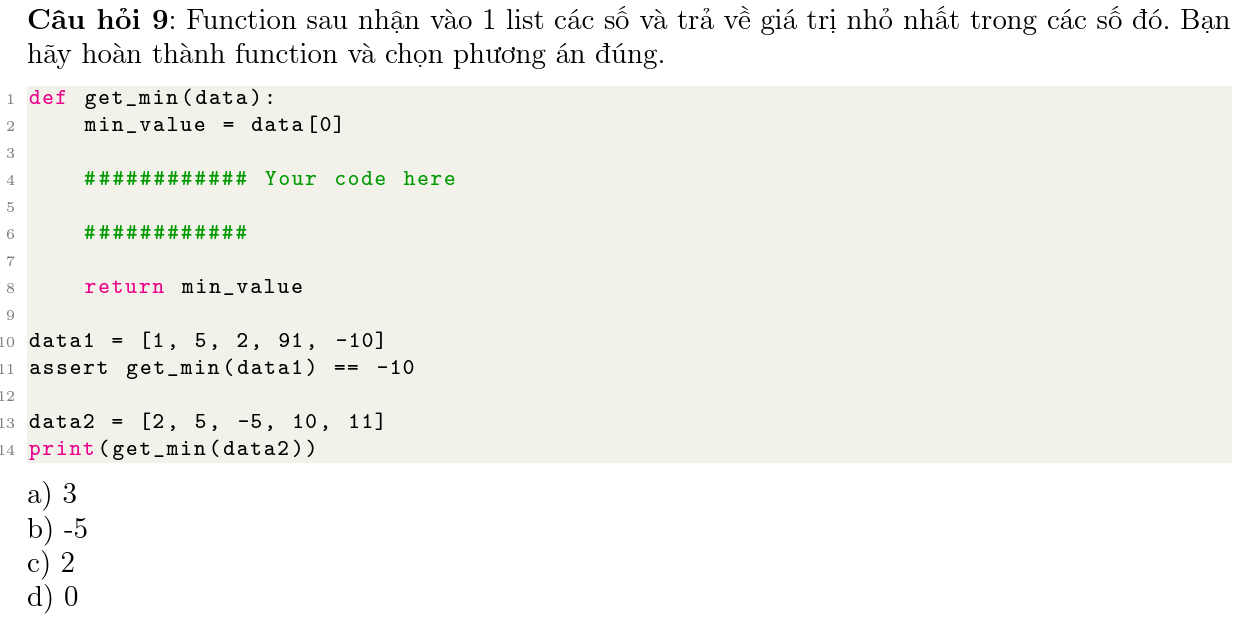
\includegraphics[width=1\linewidth]{image1.png}
    \label{fig:enter-label}
\end{figure}

\begin{figure}[H]
    \centering
    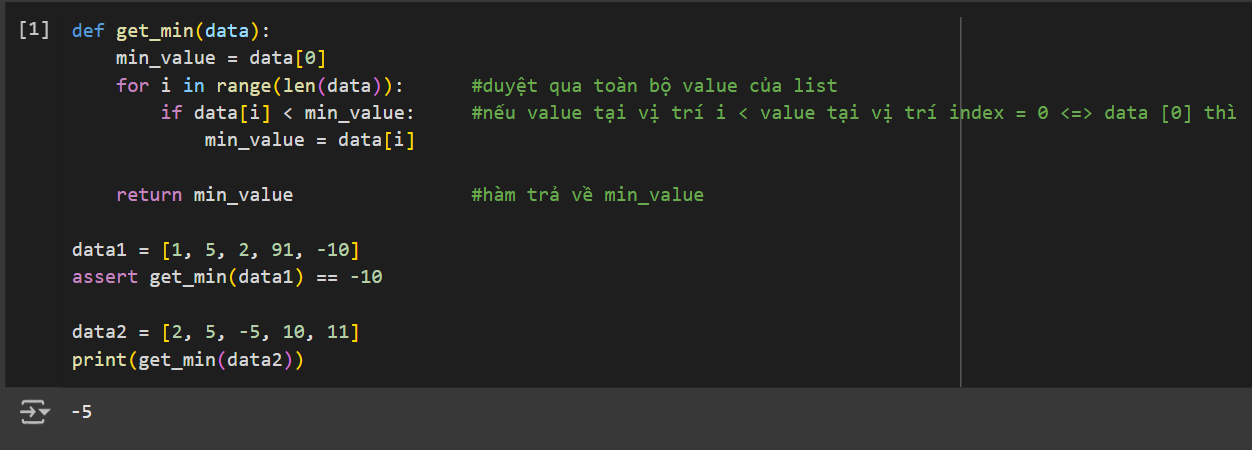
\includegraphics[width=1\linewidth]{image2.png}
    \label{fig:enter-label}
\end{figure}

\clearpage
\begin{figure}[H]
    \centering
    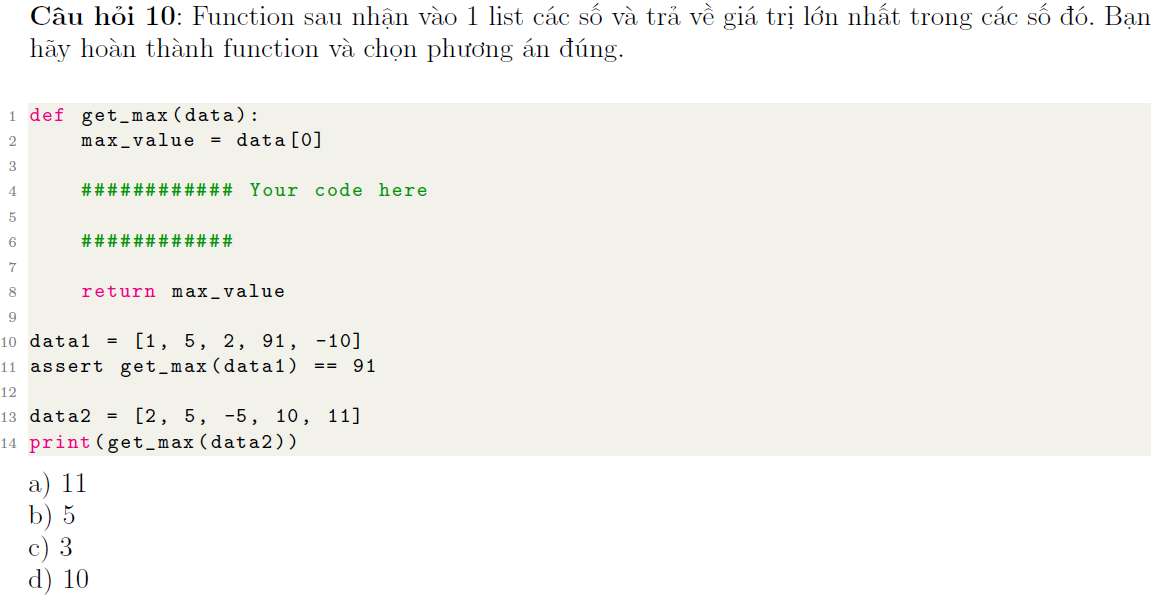
\includegraphics[width=1\linewidth]{image3.png}
    \label{fig:enter-label}
\end{figure}

\begin{figure}[H]
    \centering
    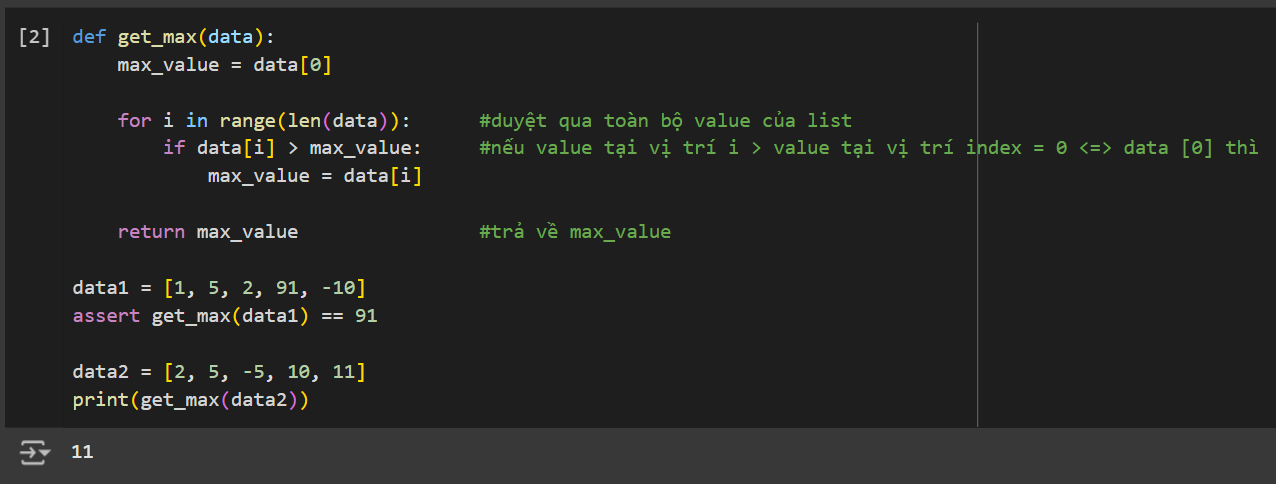
\includegraphics[width=1\linewidth]{image4.png}
    \label{fig:enter-label}
\end{figure}

\clearpage
\begin{figure}[H]
    \centering
    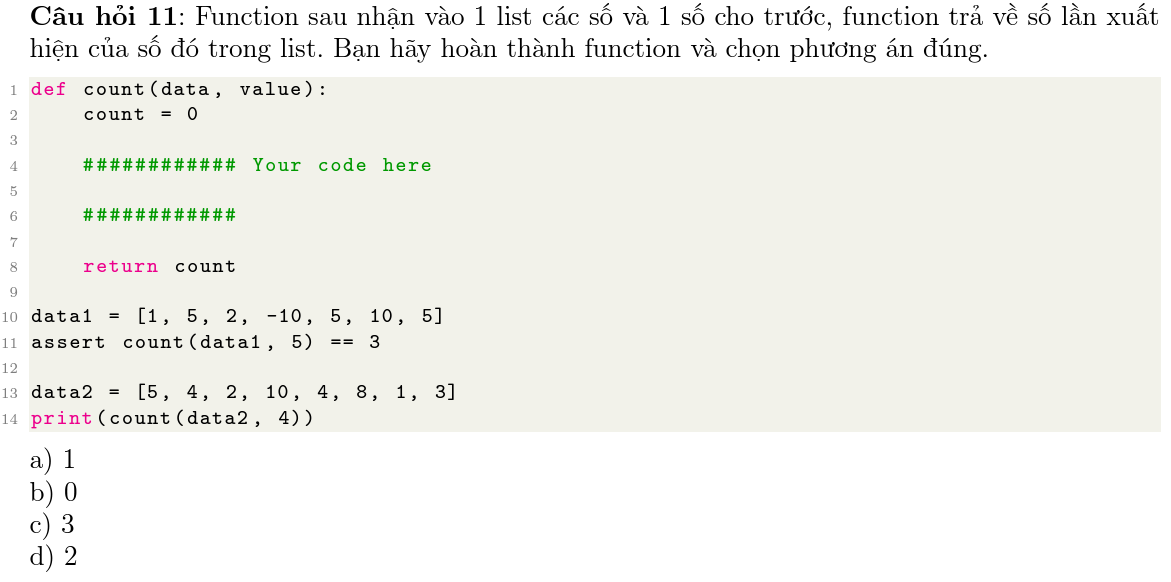
\includegraphics[width=1\linewidth]{image5.png}
    \label{fig:enter-label}
\end{figure}

\begin{figure}[H]
    \centering
    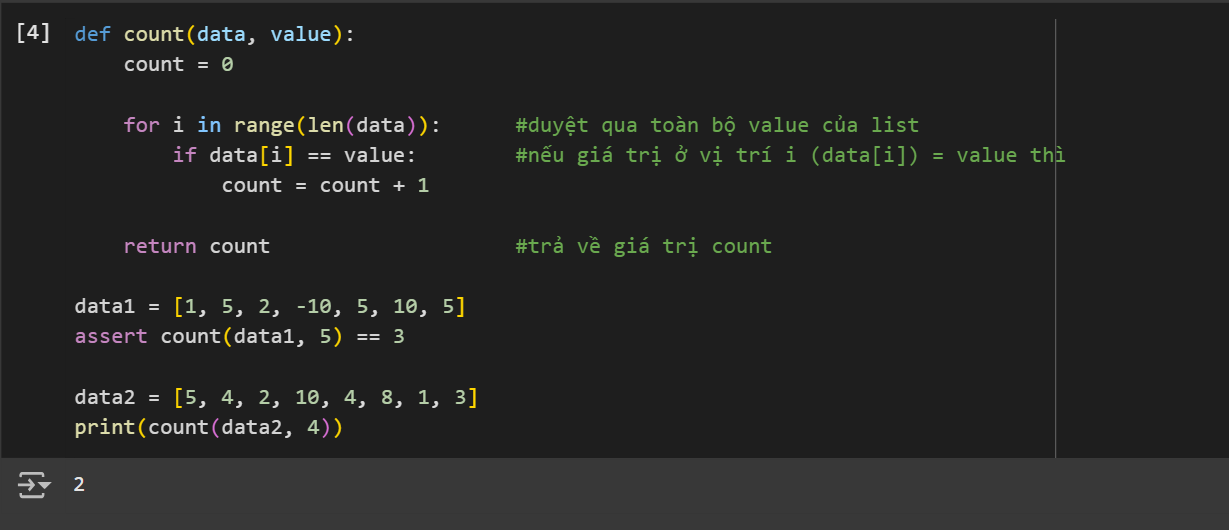
\includegraphics[width=1\linewidth]{image6.png}
    \label{fig:enter-label}
\end{figure}

\clearpage
\begin{figure}[H]
    \centering
    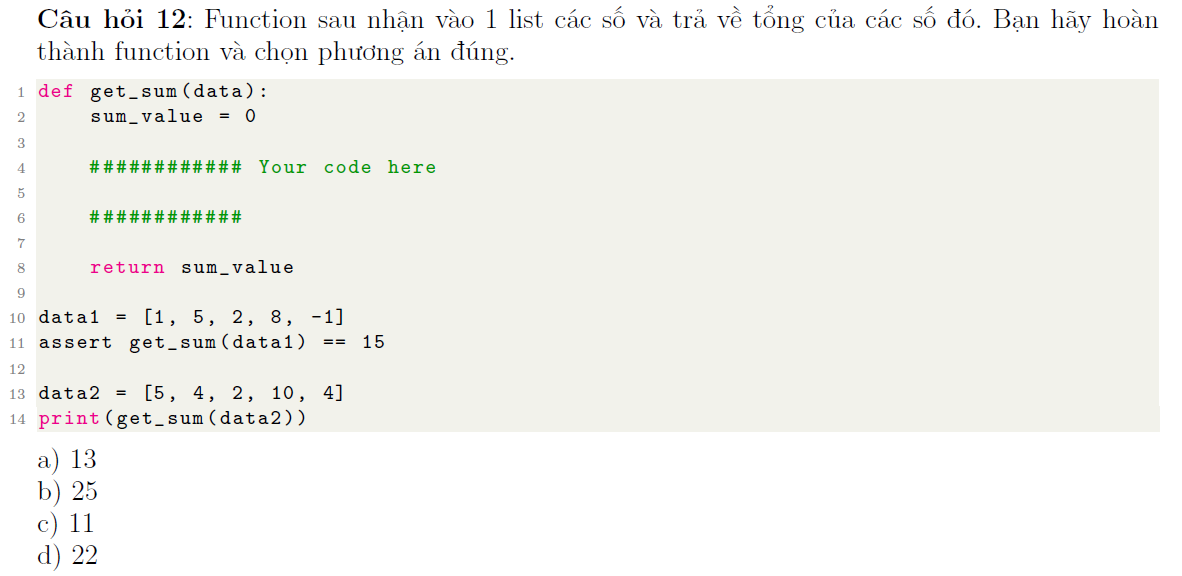
\includegraphics[width=1\linewidth]{image7.png}
    \label{fig:enter-label}
\end{figure}

\begin{figure}[H]
    \centering
    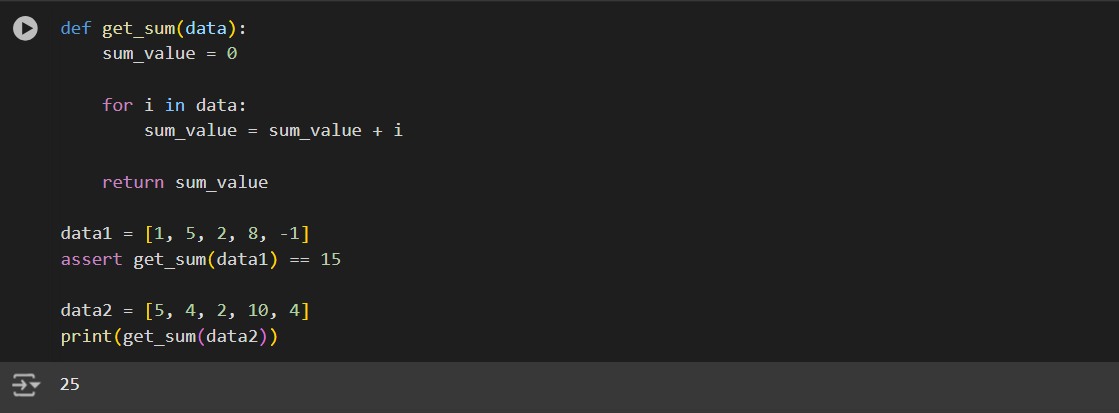
\includegraphics[width=1\linewidth]{image8.png}
    \label{fig:enter-label}
\end{figure}

\begin{figure}[H]
    \centering
    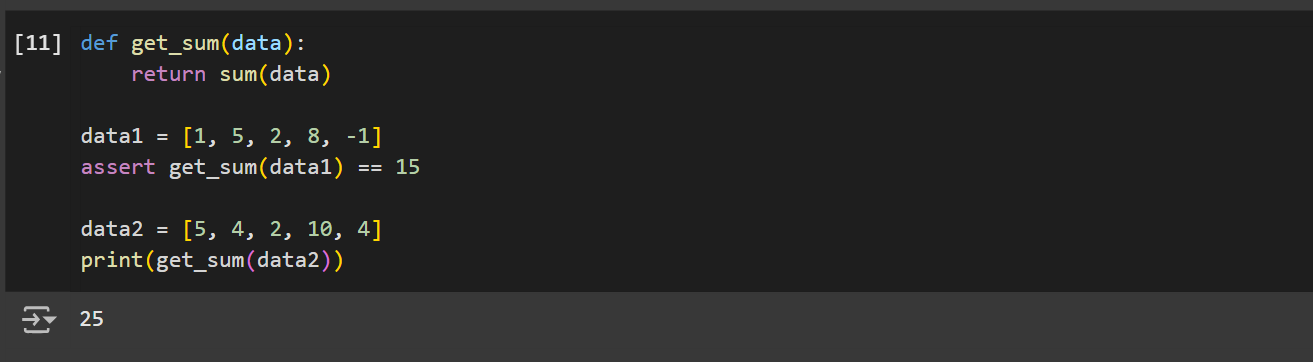
\includegraphics[width=1\linewidth]{image.png}
    \label{fig:enter-label}
\end{figure}

\clearpage
\begin{figure}[H]
    \centering
    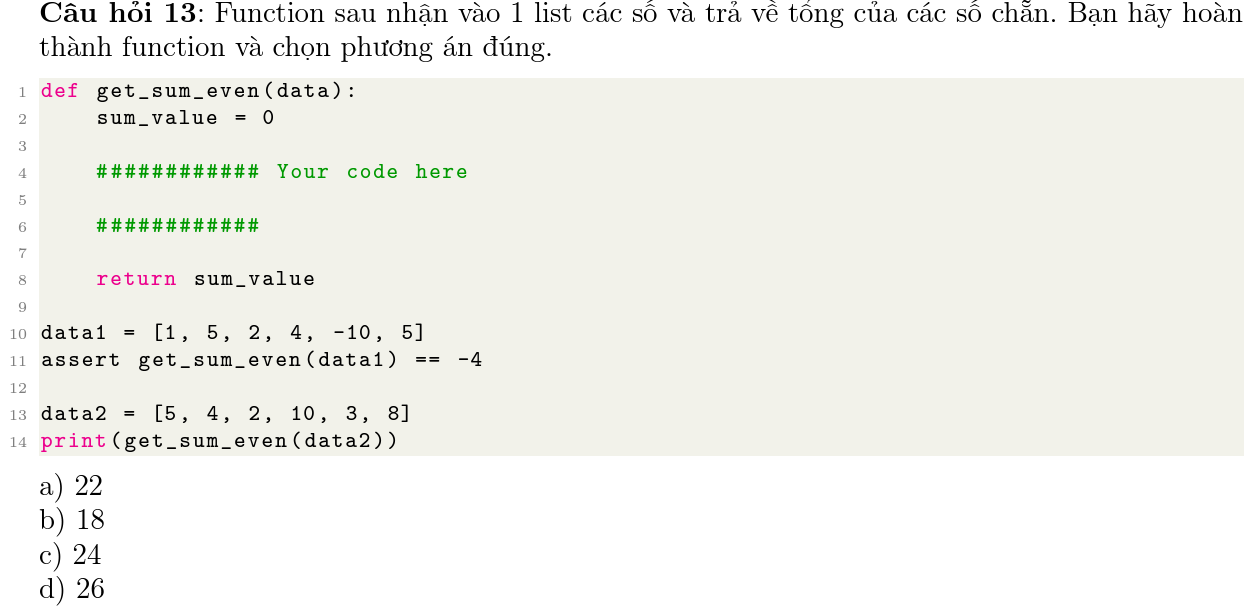
\includegraphics[width=1\linewidth]{image9.png}
    \label{fig:enter-label}
\end{figure}

\begin{figure}[H]
    \centering
    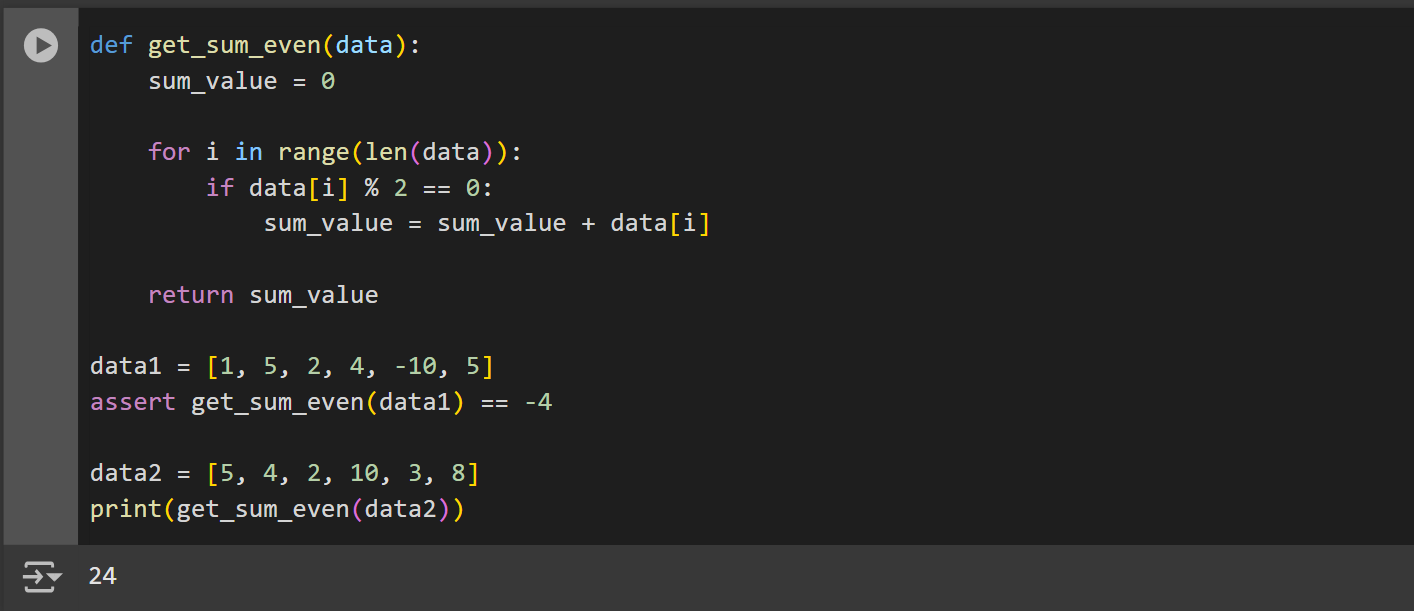
\includegraphics[width=1\linewidth]{image10.png}
    \label{fig:enter-label}
\end{figure}

\begin{figure}[H]
    \centering
    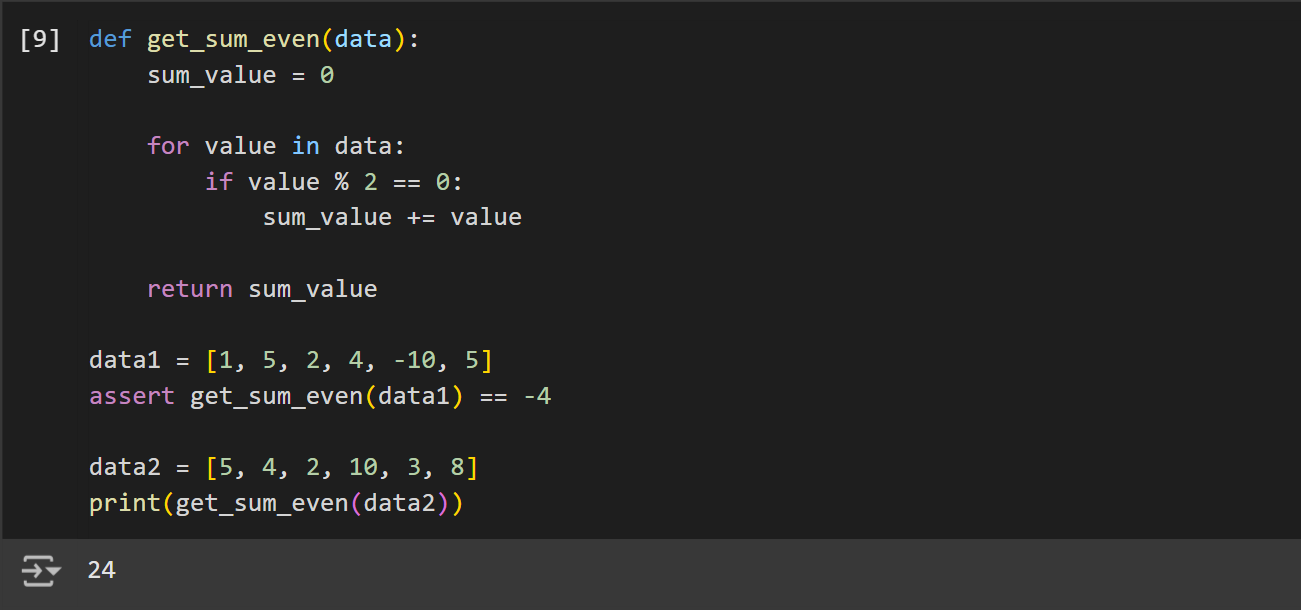
\includegraphics[width=1\linewidth]{image11.png}
    \label{fig:enter-label}
\end{figure}

\clearpage
\begin{figure}[H]
    \centering
    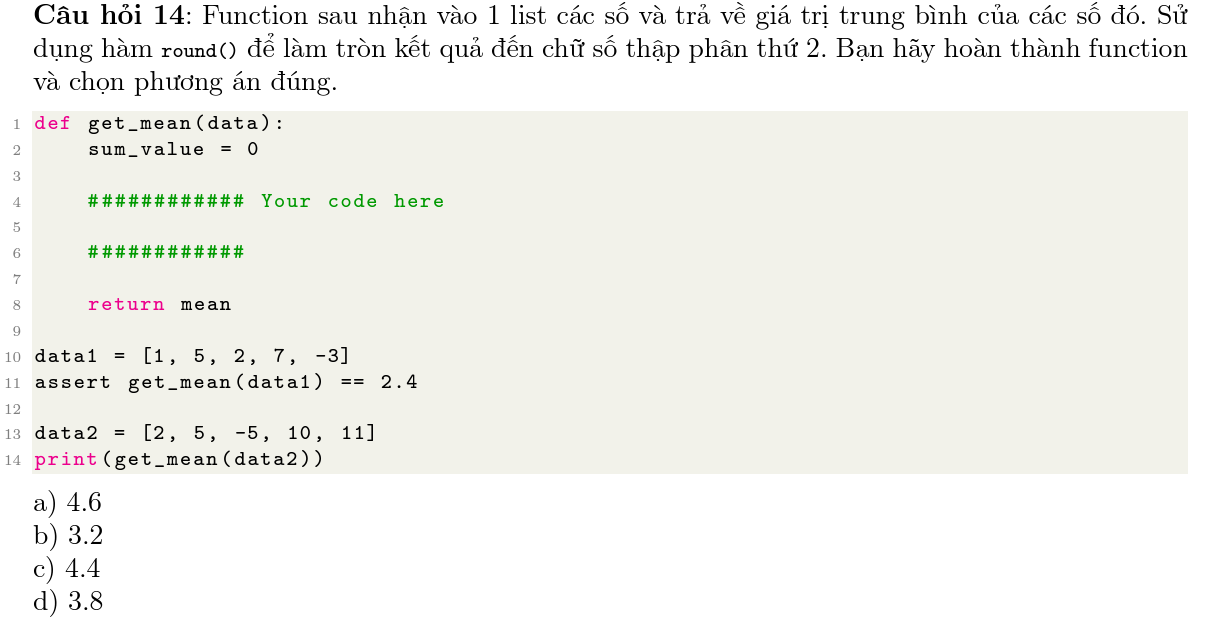
\includegraphics[width=1\linewidth]{image12.png}
    \label{fig:enter-label}
\end{figure}

\begin{figure}[H]
    \centering
    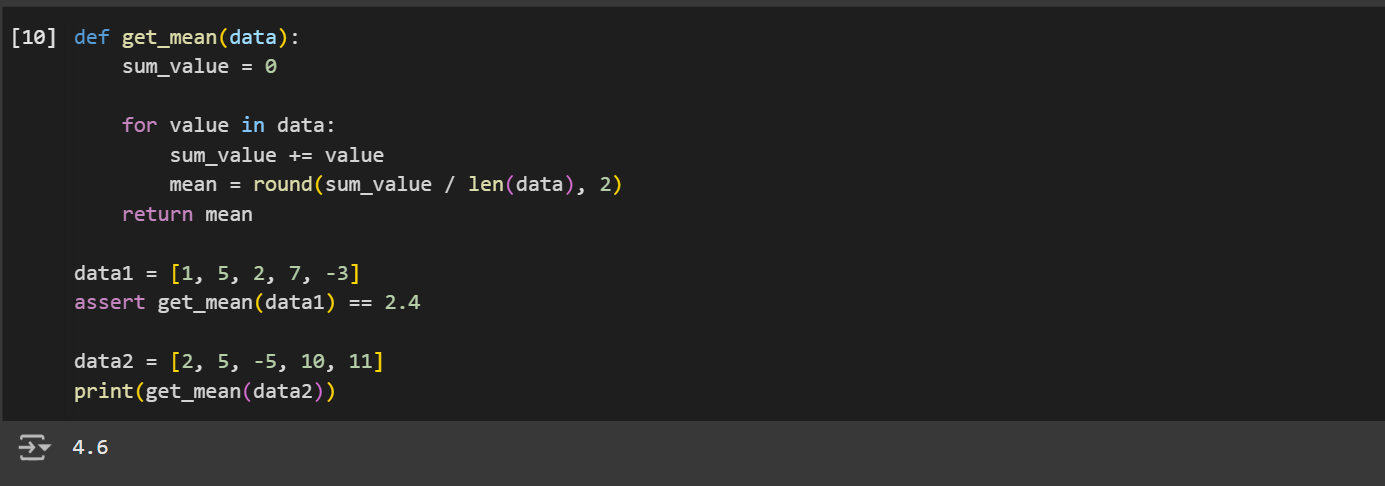
\includegraphics[width=1\linewidth]{image13.png}
    \label{fig:enter-label}
\end{figure}

\begin{figure}[H]
    \centering
    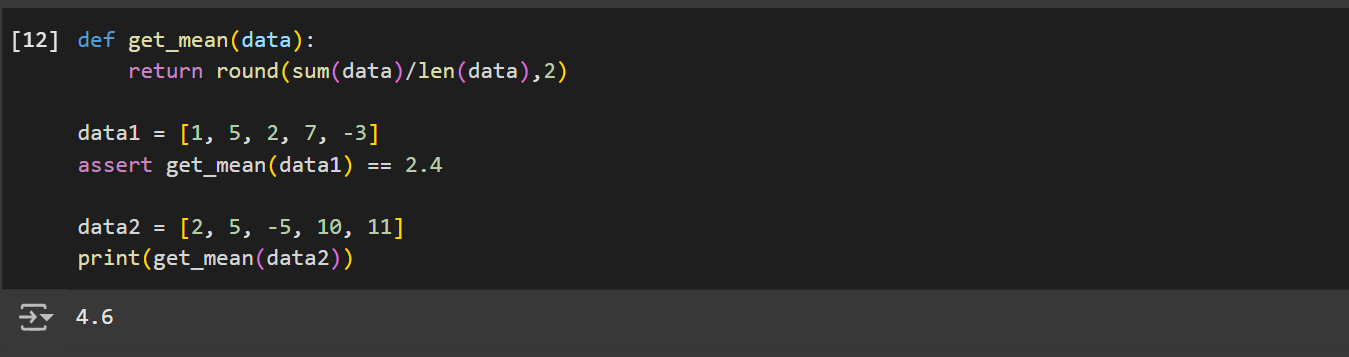
\includegraphics[width=1\linewidth]{image14.png}
    \label{fig:enter-label}
\end{figure}

\clearpage
\begin{figure}[H]
    \centering
    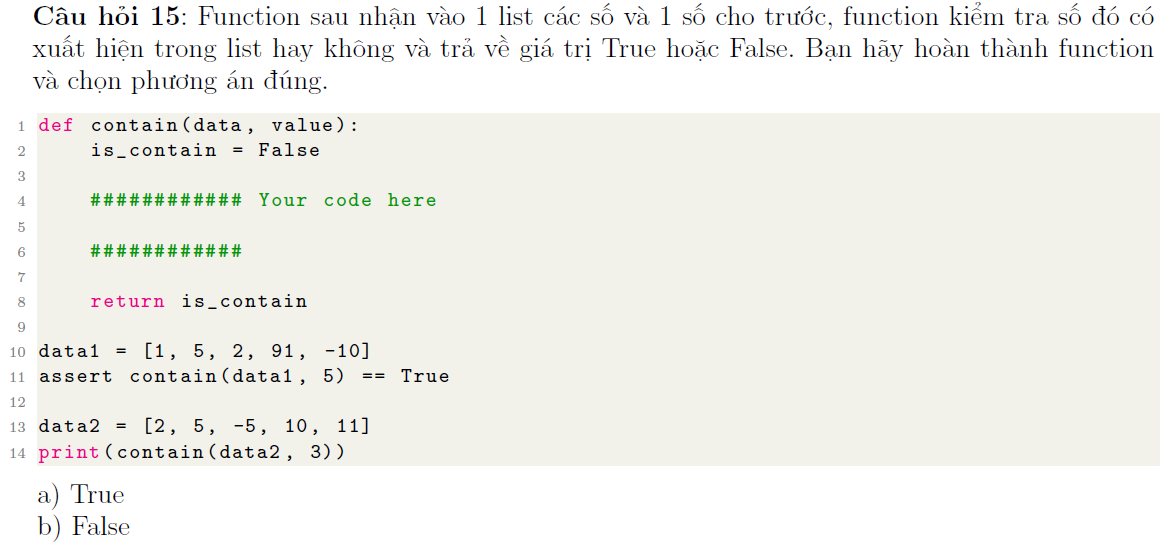
\includegraphics[width=1\linewidth]{15.png}
    \label{fig:enter-label}
\end{figure}

\begin{figure}[H]
    \centering
    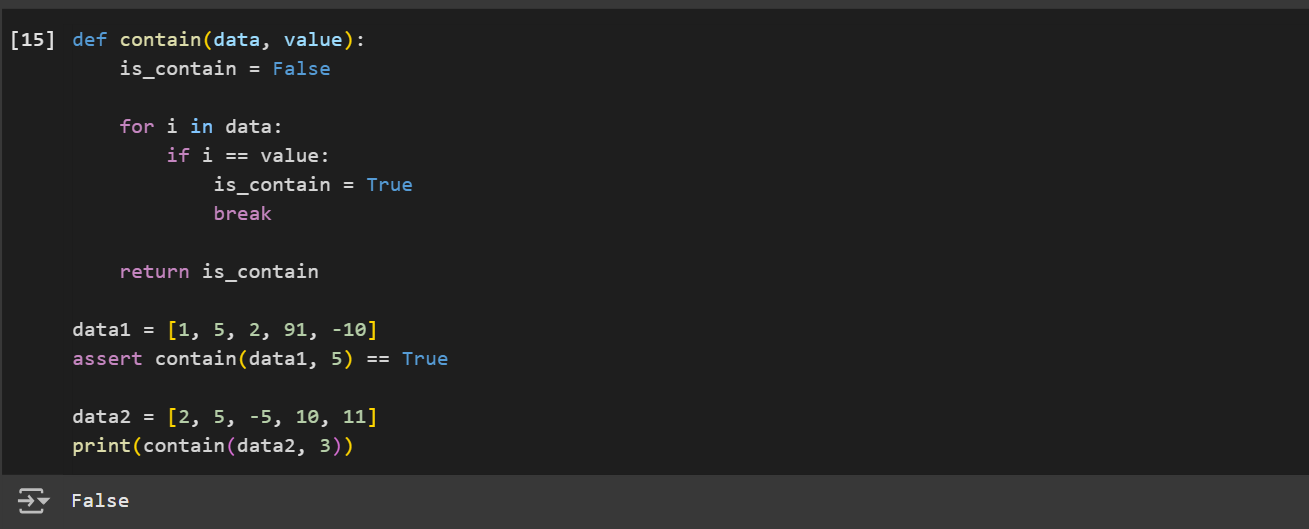
\includegraphics[width=1\linewidth]{16.png}
    \label{fig:enter-label}
\end{figure}

\begin{figure}[H]
    \centering
    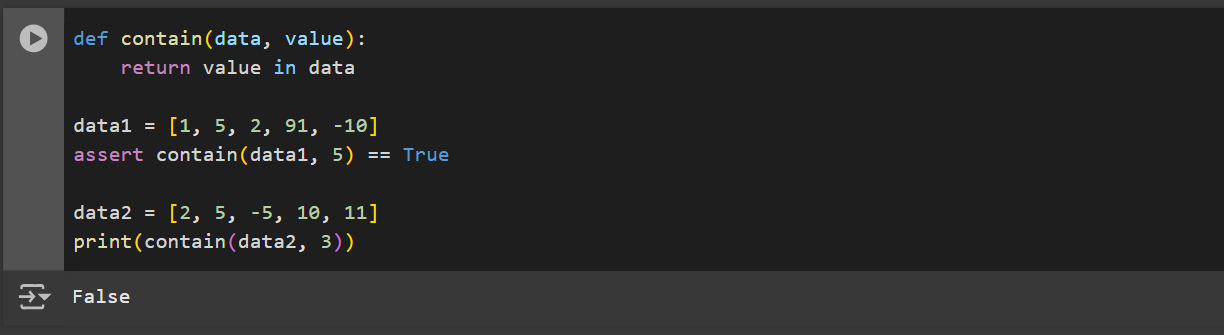
\includegraphics[width=1\linewidth]{17.png}
    \label{fig:enter-label}
\end{figure}

\clearpage
\section{Interpolation in image resizer}
\begin{figure}[H]
    \centering
    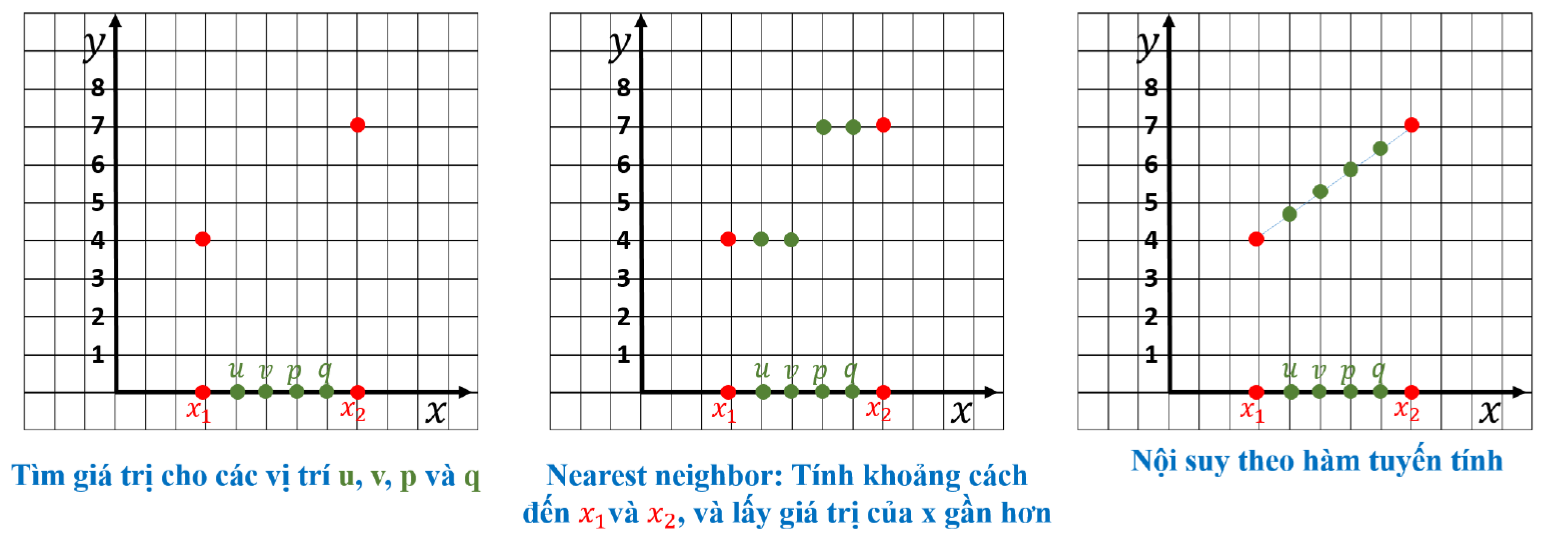
\includegraphics[width=1\linewidth]{18.png}
    \label{fig:enter-label}
\end{figure}

\subsection{Nearest neighbor}
Khi bạn muốn nội suy giá trị tại một vị trí chưa được biết, NN tìm điểm dữ liệu có khoảng cách gần nhất đến vị trí đó và sử dụng giá trị của điểm gần nhất này. 
\par
\vspace{10pt}
NN thích hợp để scale hình ảnh hoặc dữ liệu khi độ chính xác không phải là ưu tiên cao.
Thường xử lý dữ liệu không liên tục hoặc có tính chất phân đoạn vì ưu điểm nhanh và dễ thực hiện
\par
\vspace{10pt}
Bài toán đặt ra là từ một ma trận 3x3 chuyển thành một ma trận 6x6 
\begin{figure}[H]
    \centering
    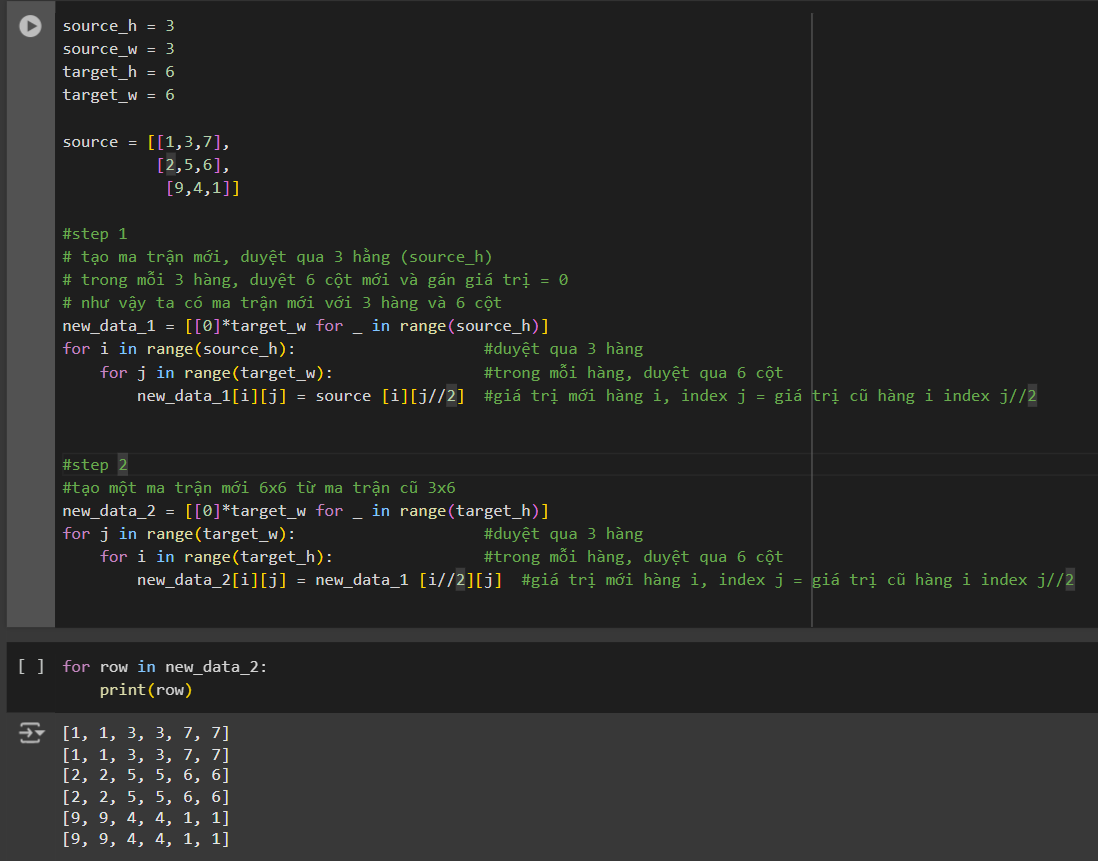
\includegraphics[width=0.9\linewidth]{19.png}
    \label{fig:enter-label}
\end{figure}

\clearpage
\subsection{Linear interpolation}
Linear interpolation (nội suy tuyến tính) sử dụng phương trình đường thẳng để ước tính giá trị giữa hai điểm dữ liệu đã biết.
\par
\vspace{10pt}
Với 2 điểm $x_1,y_1$ và $x_2,y_2$ cho trước, giá trị $y$ tại một điểm $x$ bất kỳ giữa $x_1$ và $x_2$ được tính theo công thức:
\begin{center}
\large
    $y = y_1 + \frac{(x-x_1)}{(x_2-x_1)}.(y_2-y_1)$
\end{center}
Bài toán đặt ra: trong một list, tìm cách vị trí None và sử dụng linear interpolation để điền vào các giá trị 
\begin{figure}[H]
    \centering
    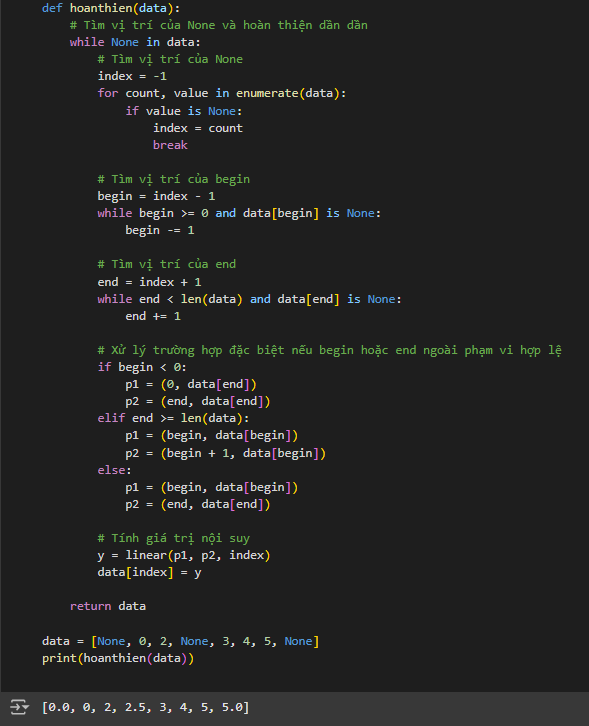
\includegraphics[width=0.9\linewidth]{21.png}
    \label{fig:enter-label}
\end{figure}
\end{document}
